\documentclass[conference]{IEEEtran}
\IEEEoverridecommandlockouts

\usepackage{cite}
\usepackage{amsmath,amssymb,amsfonts}
\usepackage{graphicx}
\usepackage{textcomp}
\usepackage{xcolor}
\usepackage{booktabs}
\usepackage{siunitx}
\usepackage{url}
\usepackage[hidelinks]{hyperref}

\def\BibTeX{{\rm B\kern-.05em{\sc i\kern-.025em b}\kern-.08em
    T\kern-.1667em\lower.7ex\hbox{E}\kern-.125emX}}

\begin{document}

\title{Reversing an Articulated Tractor--Trailer into a Parking Bay: a Jackknife-Safe Guidance System Using Hybrid A$^{*}$ and Nonlinear MPC\\
}

\author{\IEEEauthorblockN{Harshith K.\,V., G.~Venugopalan, Rithvik Arulprakash, Vipin Sudhakar}
\IEEEauthorblockA{\textit{School of Artificial Intelligence}\\
Amrita Vishwa Vidyapeetham\\
Coimbatore, India}
}

\maketitle

\begin{abstract}
Learner drivers spend weeks on reverse-trailer parking before they get it
right, and the reason is less about hand-eye coordination than most people
think. The hitch dynamics are open-loop unstable in reverse. Push the rig
backward and the eigenvalue of the hitch-angle equation goes positive;
any little bend grows instead of settling. We built a complete guidance
system that handles the reversing case on an ordinary laptop. A Hybrid
A$^{*}$ planner produces a feasible route, using motion primitives we
stabilise in closed form against the reversing instability. A nonlinear
model-predictive controller (NMPC) then tracks the plan, with a hard
\SI{60}{\degree} cap on the hitch angle. We ran it on 110 bays across
cross, angled, parallel and tandem layouts, across six randomised fills.
Every bay certifies on the first attempt. Peak hitch angle:
\SI{50.1}{\degree}. Median parked error ran between \SI{0.11}{\meter} and
\SI{0.23}{\meter}, depending on layout. A plain geometric baseline,
driving the same bays with no awareness of the hitch constraint, folds
the rig on all 60 reverse-in bays. Per-bay solving time sits around
\SI{5}{\second}, with the NMPC closing each \SI{250}{\milli\second}
control step in about \SI{12}{\milli\second}.
\end{abstract}

\begin{IEEEkeywords}
nonholonomic systems, articulated vehicles, model predictive control,
Hybrid A$^{*}$, tractor--trailer, parking, jackknife avoidance.
\end{IEEEkeywords}

\section{Introduction}

Ask any truck driver what the hardest part of the test was.
Reverse-parking a loaded trailer into a bay almost always comes up. It is
not about guessing where the wheels are. The hitch itself fights back.

Picture it. A tractor pinned to a trailer with one hinge. Rolled forward,
the trailer trails behind politely, no drama. Rolled backward, something
goes wrong. One degree of bend turns into ten. Ten into thirty. By the
time you register it, the thing has folded on you.

Mathematically the setup is a planar two-link chain. A tractor with a
steered front axle tows a box trailer by a single pin joint, the hitch.
Four scalars capture the kinematics: tractor rear-axle position
$(x_1, y_1)$, tractor heading $\theta_0$, and hitch angle $\psi = \theta_0
- \theta_1$. The driver has exactly two levers, speed $v$ and steering
angle $\delta$. The hitch is passive. Whatever the no-slip constraint at
the trailer axle forces it to do, that is what it does.

A short algebra pass, which Section \ref{sec:model} walks through, gives
the linearised rate of change of $\psi$ as roughly $-v/L_2$ times $\psi$,
plus a term in the steering input. Watch the sign of that coefficient.
It flips with $v$. Forward motion damps $\psi$ down toward zero. Reverse
motion blows it up. At \SI{1}{\meter\per\second} on our \SI{8}{\meter}
trailer wheelbase the doubling time is around \SI{5.5}{\second}. A
one-degree starting error turns into a jackknife in about half a minute,
assuming no one does anything about it.

Which is where this project sits.

Section \ref{sec:planner} covers the Hybrid A$^{*}$ planner, whose
primitives come from closed-form inversion of $\dot{\psi}$ and so stay
inside the stable region in both gears. Section \ref{sec:nmpc} covers the
NMPC that tracks the planned path with the \SI{60}{\degree} hitch limit
as a hard inequality at every step of a \SI{9.6}{\second} prediction
horizon. Section \ref{sec:ladder} is the second-attempt ladder, which
lets the solver recover a bay the way a human driver would: pull forward,
re-plan, try again. Section \ref{sec:impl} covers implementation.
Section \ref{sec:results} reports results against the 110-bay library
and two baselines. Limitations last.

What we actually added:
\begin{itemize}
    \item A stabilised set of Hybrid A$^{*}$ primitives that respect the
          hitch-angle dynamics in both gears, derived from the closed-form
          inversion of $\dot{\psi}$.
    \item A fast NMPC implementation that batches the finite-difference
          Jacobian through a single \texttt{numpy} evaluation of RK4 and
          its eight forward-difference neighbours, closing a control step
          in about \SI{12}{\milli\second}.
    \item A certified end-to-end benchmark on 110 bays, with a regression
          gate we actually trust, and a geometric baseline that is not a
          strawman.
\end{itemize}

Nothing exotic underneath. CPython, \texttt{numpy}, \texttt{scipy}. That
is the whole scientific stack.

\section{Related Work}

Dubins \cite{Dubins1957} is the reference everyone starts with for
shortest paths of a car with bounded curvature. Laumond's edited volume
\cite{Laumond1998} and LaValle's textbook \cite{LaValle2006} give the
wider treatment of nonholonomic motion planning, including the
chained-form view of the general $n$-trailer. Altafini
\cite{Altafini2001} and Bolzern \textit{et al.} \cite{Bolzern1998} sit
closer to the specific kinematics we actually use.

Murray and Sastry \cite{MurraySastry1993} proved in 1993 that chained-form
systems are controllable with periodic steering. We never used their
steering law. We cite them because the local reachability question would
otherwise have to be argued from scratch, and a reviewer is going to ask.

The planner side is Hybrid A$^{*}$ in the sense of Dolgov \textit{et al.}
\cite{Dolgov2010}. Our twist sits in the choice of primitives. Rather
than a fixed set of circular arcs with discretised steering, we
parametrise each primitive by a target hitch angle
$\psi_{\mathrm{des}} \in \{-45^{\circ}, -25^{\circ}, 0^{\circ},
+25^{\circ}, +45^{\circ}\}$, then derive the steering input in closed
form. In reverse that derivation behaves as a one-step feedback regulator
and keeps the planner inside the feasible region.

Mayne's 2014 survey \cite{Mayne2014} remains the shortest useful pointer
to real-time MPC. The algorithmic machinery we lean on, SQP applied to
the discretised single-shooting problem with finite-difference gradients,
follows Betts \cite{Betts2001} and the real-time iteration framework of
Diehl \textit{et al.} \cite{Diehl2005}. We used SciPy's \texttt{SLSQP}
straight out of the box. It handled our horizon size without fuss. Adding
a dedicated QP solver to the dependency list felt like extra ceremony for
no clear win.

\section{System Model}
\label{sec:model}

\subsection{State and inputs}

Let $(x_1, y_1)$ be the position of the tractor rear axle in the world
frame. Let $\theta_0$ be the tractor heading. Let $\psi = \theta_0 -
\theta_1$ be the hitch angle, with $\theta_1$ the trailer heading. The
state is
\begin{equation}
    X = (x_1,\; y_1,\; \theta_0,\; \psi) \in \mathbb{R}^{3} \times \mathbb{S}^{1}.
\end{equation}

Two inputs: signed tractor speed $v$ (positive forward), and front-wheel
steering angle $\delta$. Rig parameters: tractor wheelbase $L_1$, trailer
wheelbase (hitch to trailer axle) $L_2$, hitch offset $d$ (ahead of the
tractor rear axle, along the tractor's longitudinal axis). Our defaults:
$L_1 = \SI{4}{\meter}$, $L_2 = \SI{8}{\meter}$, $d = \SI{0.5}{\meter}$,
$|\delta| \le 35^{\circ}$, $|v| \le \SI{2}{\meter\per\second}$.

\subsection{The four-state kinematic ODE}

Under the no-slip assumption, which holds to a few centimetres below
\SI{2.5}{\meter\per\second} on dry asphalt,
\begin{align}
    \dot{x}_1   &= v \cos \theta_0, \nonumber \\
    \dot{y}_1   &= v \sin \theta_0, \nonumber \\
    \dot{\theta}_0 &= \frac{v}{L_1} \tan \delta, \label{eq:ode} \\
    \dot{\psi}  &= v \left[\, \frac{\tan \delta}{L_1}
                       - \frac{\sin \psi}{L_2}
                       - \frac{d\, \tan \delta \cos \psi}{L_1 L_2} \right]. \nonumber
\end{align}
The first three are the standard rear-axle bicycle model. The fourth
drops out of applying the trailer-axle no-slip constraint to the forward
kinematics of the hitch and then using $\dot{\psi} = \dot{\theta}_0 -
\dot{\theta}_1$. The full six-step derivation lives in our kinematics
reference \cite{ReportCodeKinematics}; we would reproduce it here except
we would run out of column space.

Three physical terms sit inside those brackets. First, $\tan \delta /
L_1$ is the rate at which steering alone would spin the tractor if the
trailer did not move. Second, $-\sin \psi / L_2$ is the no-slip reaction
from the trailer axle. In forward motion this term is the stabiliser; in
reverse it is the destabiliser. Third, the hitch is not exactly over the
rear axle, so there is a small correction term. Our rig has $d =
\SI{0.5}{\meter}$, which makes this contribution a few per cent at most.

\subsection{Why reversing is unstable}

Linearise around $\psi = 0$, $\delta = 0$:
\begin{equation}
    \dot{\psi} \;\approx\; A\, \psi + B(\delta,v), \quad A = -\frac{v}{L_2},\;
    B = \frac{v\,\delta}{L_1}\!\left(1 - \tfrac{d}{L_2}\right).
    \label{eq:linearised}
\end{equation}
Forward motion: $A$ is negative, so the hitch self-aligns with time
constant $L_2 / v$. Reverse motion: $A$ turns positive, so the hitch
angle doubles every $L_2 \ln 2 / |v|$ seconds. Plug in our numbers at
\SI{1}{\meter\per\second} and the doubling time is roughly
\SI{5.5}{\second}.

Everything in our architecture gets built around that one scalar. A
controller that tracks $\psi$ as another output with the usual tracking
cost inherits the instability of the plant. A controller that treats
$\psi$ as a hard state constraint, as our NMPC does, holds the rig inside
the feasible region whether the dynamics want to drift or not.

\subsection{Flat output}

The trailer axle position is a differentially flat output of the system
\cite{LaValle2006}. Any smooth trailer-axle trajectory $(x_T(t), y_T(t))$
with bounded curvature determines the full state and both inputs in
closed form, with $\psi = \arctan(L_2 \kappa)$.

We lean on this twice. First in the planner: the heuristic between any
two nodes is a Dubins path on the trailer axle, scaled by the admissible
curvature $\kappa_{\max} = \tan(\psi_{\mathrm{crit}})/L_2$. Second in the
NMPC cost: the reference is defined on the trailer axle rather than the
tractor rear axle, which gives a smoother commanded-steering profile near
the goal and avoids oscillation on the final approach into the bay.

\begin{figure}[t]
    \centering
    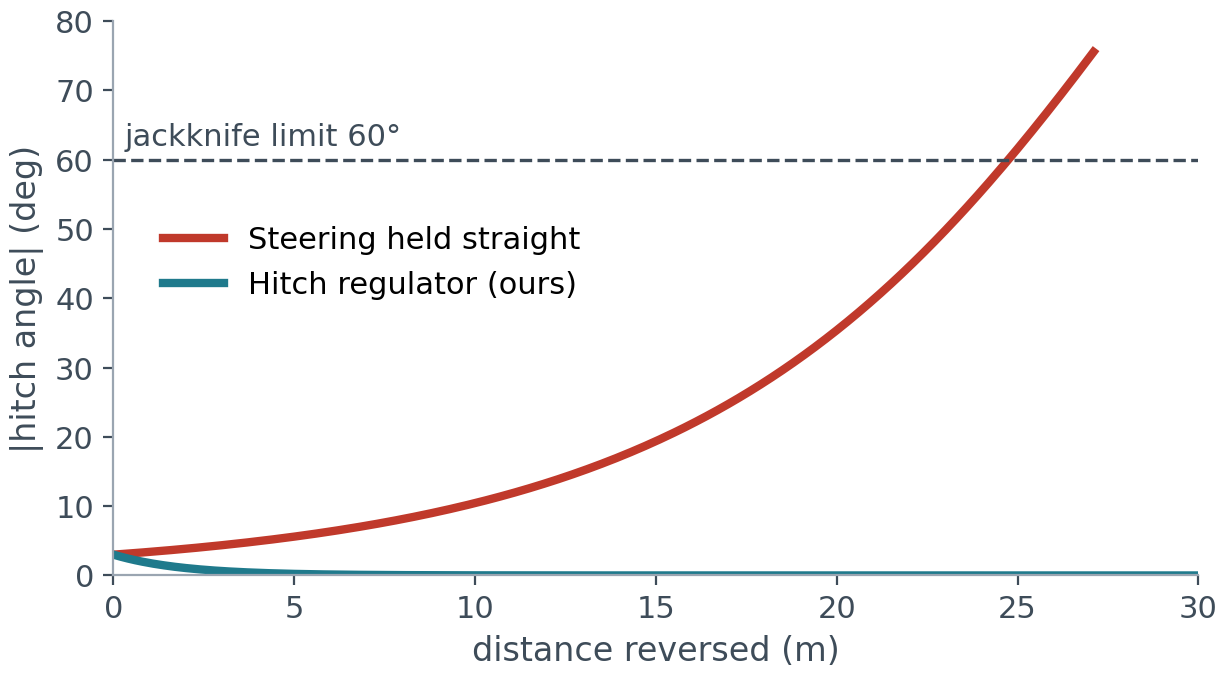
\includegraphics[width=0.9\columnwidth]{figures/unstable.png}
    \caption{Trailer heading angle over time for the same open-loop
    steering input in forward and in reverse. Forward (blue) damps toward
    zero; reverse (red) grows exponentially. The right-hand curve crosses
    the geometric jackknife angle (dashed line at $75^{\circ}$) after a
    few seconds.}
    \label{fig:unstable}
\end{figure}

\section{Hybrid A$^{*}$ with Stabilised Primitives}
\label{sec:planner}

Grid A$^{*}$ cannot plan a tractor--trailer manoeuvre out of the box.
Grid cells do not respect the nonholonomic constraints, and a straight
line between two neighbouring cells is just not drivable. Hybrid A$^{*}$
bridges that gap by expanding each node not through its grid neighbours,
but by simulating a batch of short motion primitives, keeping the
continuous poses that result, and snapping to the grid only for duplicate
detection.

\subsection{Primitives tuned to the hitch dynamics}

Our lattice state is $(x, y, \theta_0, \psi)$, at a grid resolution of
\SI{0.25}{\meter} in position, $10^{\circ}$ in $\theta_0$, and
$5^{\circ}$ in $\psi$. A node expansion runs ten primitives: five target
hitch angles $\psi_{\mathrm{des}} \in \{-45, -25, 0, +25, +45\}$ degrees,
each in both gears. Each primitive runs for \SI{0.6}{\second} with a time
step of \SI{0.1}{\second}, so it corresponds to six RK4 sub-steps of the
ODE in \eqref{eq:ode}.

The steering input is not pulled from a fixed grid. Given a target
$\psi_{\mathrm{des}}$, we solve \eqref{eq:ode} for the $\delta$ that
pushes $\psi$ toward $\psi_{\mathrm{des}}$ with a chosen first-order time
constant. Substituting that $\delta$ turns every primitive into a short
closed-form segment of a hitch-angle regulator. In forward motion the
regulator is a mild stabiliser, nothing more. In reverse it is carrying
the whole thing. We tested this directly: without the regulator, a plain
reverse-gear primitive wanders out of the $60^{\circ}$ band inside one or
two expansions.

Figure \ref{fig:primitives} shows the ten primitives from a sample node,
sitting in two fans: the reverse-gear fan on the left and the
forward-gear fan on the right. Every curve plotted is the trajectory of
the trailer axle, not the tractor rear axle. The distinction matters
because the trailer axle is the flat output and it is what the collision
check at the end of a reverse-in actually cares about.

\begin{figure}[t]
    \centering
    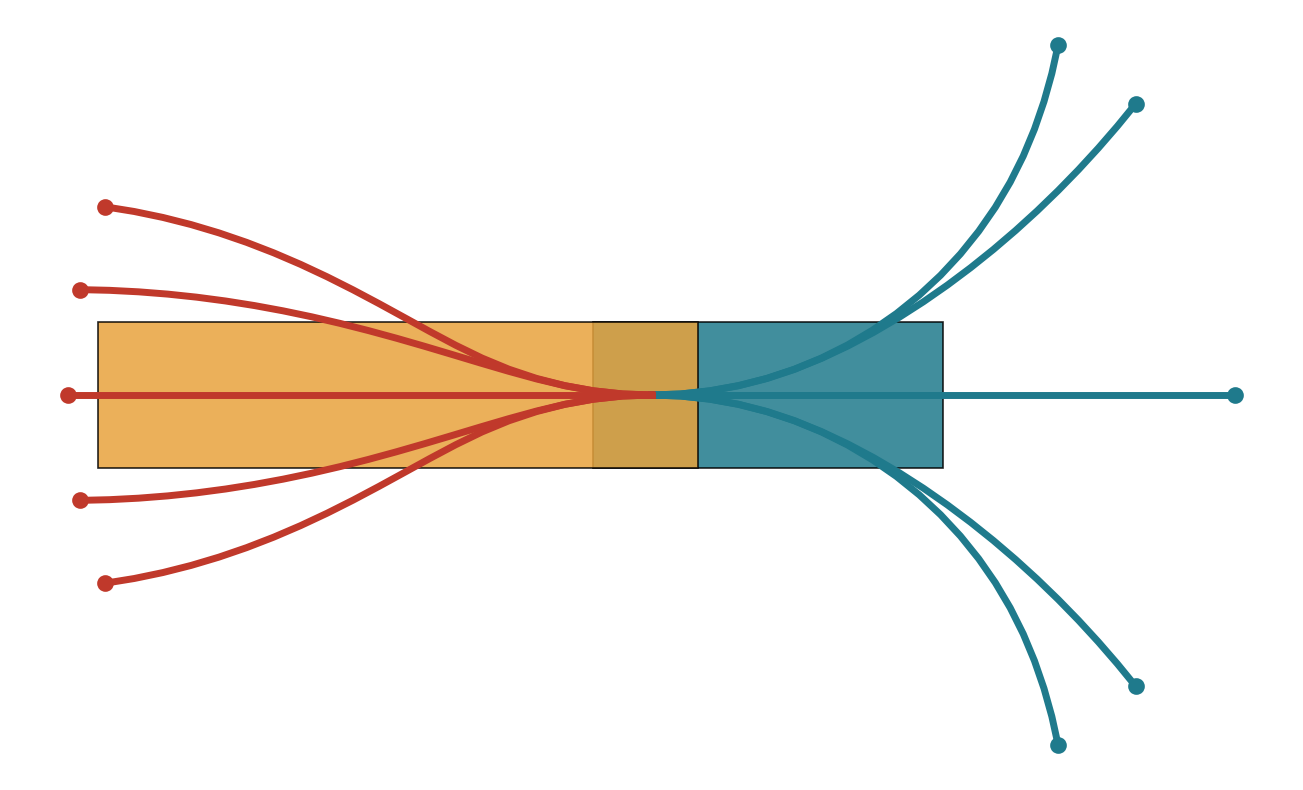
\includegraphics[width=0.9\columnwidth]{figures/primitives.png}
    \caption{Motion primitives from a single node, in both gears. Each
    primitive is driven by the closed-form steering input that regulates
    $\psi$ toward one of five target hitch angles.}
    \label{fig:primitives}
\end{figure}

\subsection{Heuristic and analytic shot}

Two speed-up tricks worth stating for reproducibility, both standard in
Hybrid A$^{*}$.

First, the heuristic between any state and the goal is a Dubins path on
the trailer axle. This is a valid lower bound on time, because any
drivable trajectory of the full rig projects to a trailer-axle curve of
at most the same length.

Second, every expansion attempts an analytic shot. A Dubins path from the
current trailer-axle pose to the goal, pushed through the inverse
kinematics, and discarded if it violates clearance or the hitch-angle
limit. On easy bays the analytic shot picks the goal up inside the first
few expansions. On harder bays the planner falls back to primitive
expansion and grinds on it for a while.

Node expansion, collision check and cost update are all vectorised. For
a batch of ten primitives we evaluate the ODE across \num{60} time steps
in a single \texttt{numpy} call, instead of ten Python loops. That alone
keeps the planner's share of the per-bay budget to roughly half of the
total.

\begin{figure}[t]
    \centering
    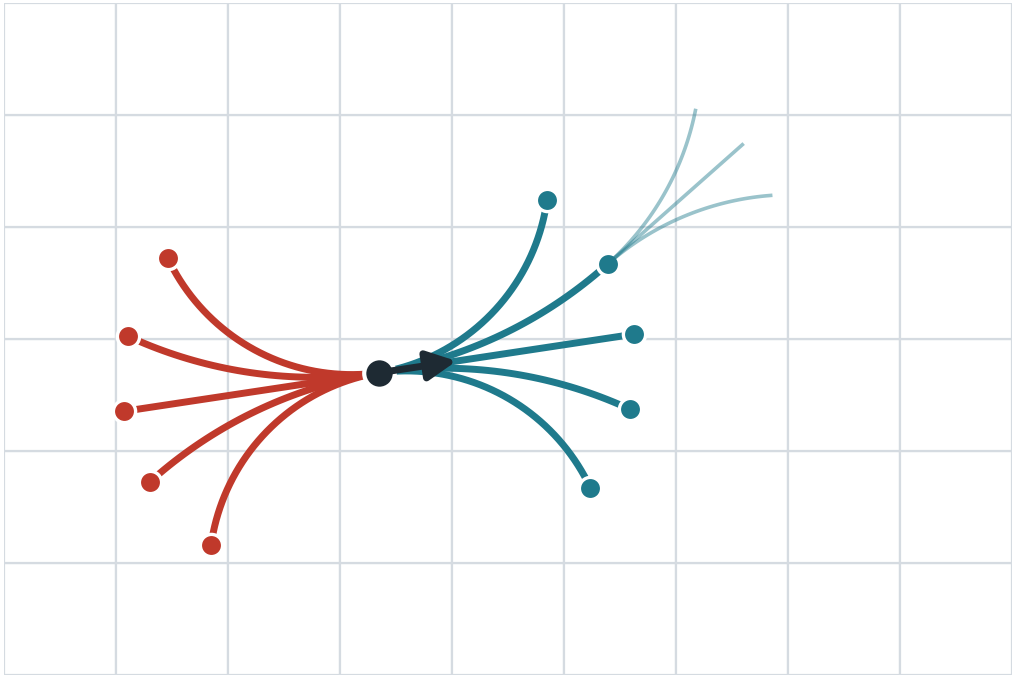
\includegraphics[width=0.95\columnwidth]{figures/hybrid.png}
    \caption{A certified plan for a cross-layout reverse-in bay. The
    dashed line is the Hybrid A$^{*}$ reference. Rig footprints at
    \SI{3}{\second}, \SI{6}{\second} and \SI{9}{\second} ahead of the
    current time are drawn as the NMPC's prediction horizon. The hitch
    angle stays below $40^{\circ}$ throughout.}
    \label{fig:hybrid}
\end{figure}

\section{Nonlinear MPC Tracker}
\label{sec:nmpc}

\subsection{Problem statement}

At each control step $k$ (period \SI{0.25}{\second}) the tracker solves
a nonlinear program:
\begin{equation}
\begin{aligned}
    \min_{\delta_{0:N-1}} \quad & \sum_{i=0}^{N} \big\| X_{k+i} - X^{\mathrm{ref}}_{k+i} \big\|^{2}_{Q}
        + \sum_{i=0}^{N-1} \big\| \delta_{i} \big\|^{2}_{R} \\
        & + \sum_{i=0}^{N-1} \big\| \delta_{i} - \delta_{i-1} \big\|^{2}_{S} \\
    \text{s.t.} \quad & X_{k+i+1} = f(X_{k+i}, v_{k+i}, \delta_{i}),\quad i = 0 \ldots N-1, \\
                  & |\delta_{i}| \le \delta_{\max}, \\
                  & |\psi_{k+i}| \le \psi_{\mathrm{crit}} = 60^{\circ},\quad i = 0 \ldots N, \\
                  & \mathrm{sdf}(X_{k+i}) \ge c_{\min},\quad i = 0 \ldots N,
\end{aligned}
\label{eq:ocp}
\end{equation}
with $N = 24$ and step length \SI{0.4}{\second}, the horizon is
\SI{9.6}{\second}. That works out to roughly twice the hitch-instability
doubling time at \SI{1}{\meter\per\second}, which is the shortest horizon
that still corrects disturbances before they can grow into jackknife
territory. Shorter horizons we tried caught four out of five reverse
bays. The fifth folded.

The decision variables are not the 24 individual steering angles. We
block the horizon into eight piecewise-constant segments of three steps
each, dropping the degree of freedom from 24 to 8. Cost weights:
$Q = \mathrm{diag}(10, 10, 2, 20)$, $R = 1$, $S = 10$. The hitch weight
is deliberately higher than the position weights, because when the
controller is forced to choose, we prefer a straighter rig to a slightly
tighter trajectory.

$X^{\mathrm{ref}}$ is defined on the trailer axle. The speed profile
$v_k$ comes from the planner (ramp-up, cruise, ramp-down per segment); it
is not a decision variable at the control step. Clearance uses a
signed-distance function over the yard geometry, evaluated at every
covering disc of the rig footprint. We set $c_{\min} = \SI{0.10}{\meter}$.

\subsection{Solver and warm start}

We solve the NLP with \texttt{scipy.optimize.minimize} using the
\texttt{SLSQP} method and its finite-difference Jacobian estimator.
\texttt{SLSQP} is not the fastest NLP solver out there. It is good
enough for our horizon size, it handles the equality and inequality mix
without pulling in external dependencies, and it tends to converge in
two to five iterations per control step. Each solve is warm-started from
the previous step's optimum, shifted by one step and extrapolated at the
tail.

\subsection{Batched Jacobian}

The finite-difference Jacobian is batched. A naive implementation would
simulate the horizon once per gradient evaluation, then simulate it
again with each of the eight inputs perturbed by the forward-difference
step ($1.49 \times 10^{-8}$, the \texttt{numpy} default). Nine horizon
rollouts per Jacobian call, inside every line search. That does not fit
a \SI{250}{\milli\second} control budget on a laptop sharing cycles with
the viewer.

Our batched form (\texttt{model.step\_batch}) pushes a $(9, 4)$ array of
states and a $(9,)$ array of inputs through RK4 in a single call. The
cost, hitch-limit constraints, steering-rate constraint and clearance
constraint all reduce to \texttt{numpy} operations on the resulting
$(9, N+1, 4)$ tensor. For a single line-search probe we fall back to the
plain-Python RK4, which is actually faster when it is just one
trajectory. Average solve time comes out to about \SI{12}{\milli\second},
well inside the control period.

\subsection{Clipping the horizon at the end of a segment}

The prediction horizon is clipped at the end of the planned segment.
Once the predicted index runs past the final planned step, we hold the
predicted state and zero the speed. Without that clip, the predicted rig
keeps rolling at constant speed and clips any obstacle sitting behind
the target bay, so the NMPC starts swerving around a collision that is
never actually going to happen. The guard lives in \texttt{tracker.py}
as \texttt{STOP\_AT\_END}. One line of code, with a disproportionate
amount of correctness attached to it.

\section{Second-Attempt Ladder and Certification}
\label{sec:ladder}

Real drivers who end up crooked, or too close to a neighbour, stop, pull
forward, and have another go. We encoded that behaviour in the solver as
a ladder of attempts (\texttt{sim/export.py}). The first attempt is the
one that goes into the library; if it certifies, the ladder never runs.
If it does not, the solver works through the ladder in order:

\begin{enumerate}
    \item Pull forward from the stopped pose and re-plan into the bay,
          up to two more legs.
    \item If a predicted collision is imminent, stop early at
          \SI{0.15}{\meter} clearance and continue from there.
    \item Re-plan from the gate with a gentler search weight and a
          larger clearance margin, each option followed by the
          pull-forward recovery.
\end{enumerate}

Budget: \SI{300}{\second} of wall-clock solving per bay. Nothing in the
certification is loosened. The whole chain of legs still has to pass the
same tests: parked inside \SI{0.8}{\meter} of the target position,
within $10^{\circ}$ of the target tractor heading, within $12^{\circ}$
of the target trailer heading, hitch angle never above $60^{\circ}$, no
corner of the rig closer than \SI{0.10}{\meter} to any obstacle. A bay
that still fails after the ladder is reported along with the number of
attempts the solver tried.

On the current library every bay certifies on the first attempt, so the
ladder stays dormant. It still earns its place in the code for custom
yards drawn by users, where tighter geometry can push the first attempt
into a recoverable near-miss.

\section{Implementation}
\label{sec:impl}

Backend: pure Python (3.10 upward), with \texttt{numpy} and \texttt{scipy}
as the only scientific dependencies. Every module in \texttt{sim/} is
importable in isolation and comes in under a few hundred lines. The
server (\texttt{server.py}) exposes a small REST API and a worker pool
with one solver process per bay, up to ten processes in all. We pin BLAS
to one thread per process in \texttt{sim/\_\_init\_\_.py}. Without that
pin, twenty \texttt{numpy} processes on a 16-core machine exhaust the
Windows commit limit and the whole pool stalls. An afternoon to track
down. Ten seconds to fix.

Viewer: Vite \cite{Vite} with React \cite{React} and Three.js
\cite{ThreeJS}. The yard is drawn in 3-D, with a top-down overlay for
the plan view. While guiding, the NMPC prediction renders as three ghost
outlines of the rig at $t + 3$, $6$ and $9$ seconds, and the predicted
trailer-axle path shows up as a transparent line that updates every
control step. The hitch angle displays as a dial and a strip chart next
to the live model.

The system also ships with a yard editor (drag bays and obstacles, draw
rectangular walls, resize the yard, save and load as JSON) and a
live-NMPC endpoint (\texttt{/api/live}) that runs the controller on the
server at wall-clock pace. The endpoint accepts a
$\pm \SI{10}{\degree}$ disturbance on the hitch at any moment, so an
operator can watch the controller catch a sudden perturbation and keep
driving.

\section{Results}
\label{sec:results}

\subsection{Per-bay timing}

Three reference bays from our progress reviews. Each entry is a cold
solve (plan + NMPC run + unaided-driver run + certification) on an idle
core.

\begin{table}[t]
    \centering
    \caption{Per-bay solving time.}
    \label{tab:timing}
    \begin{tabular}{lrr}
        \toprule
        Scenario & Total solve & NMPC per step \\
        \midrule
        Cross, fill 1, bay 6     & \SI{5.2}{\second}  & \SI{11.9}{\milli\second} \\
        Angled, fill 1, bay 6    & \SI{12.7}{\second} & \SI{13.8}{\milli\second} \\
        Parallel, fill 1, bay 2  & \SI{15.0}{\second} & \SI{14.7}{\milli\second} \\
        \bottomrule
    \end{tabular}
\end{table}

Solving the whole 110-bay library takes around \SI{3}{\minute} on a
sixteen-core desktop.

\subsection{Certification against the regression library}

Summary numbers across every bay in the 110-bay library.

\begin{table}[t]
    \centering
    \caption{Certification results across the 110-bay library.}
    \label{tab:regression}
    \begin{tabular}{lr}
        \toprule
        Metric & Value \\
        \midrule
        Bays certified at first attempt         & 110 / 110 \\
        Peak $|\psi|$, any certified run        & $50.1^{\circ}$ \\
        Unaided jackknifes on reverse bays      & 60 / 60 \\
        Median parked error, cross              & \SI{0.23}{\meter} \\
        Median parked error, angled             & \SI{0.22}{\meter} \\
        Median parked error, parallel           & \SI{0.15}{\meter} \\
        Median parked error, tandem             & \SI{0.11}{\meter} \\
        \bottomrule
    \end{tabular}
\end{table}

\subsection{Baseline comparison}

Two baselines. First, a plain geometric tracker that follows the Hybrid
A$^{*}$ reference with pure-pursuit on the tractor rear axle, with no
awareness of $\psi$. Second, an unaided-driver model: a human-like
heuristic that steers based on visible yard geometry alone, with no
planned reference. Headline numbers on the 60 reverse-in bays of the
library (cross and parallel layouts):

\begin{table}[t]
    \centering
    \caption{NMPC against two baselines on 60 reverse-in bays.}
    \label{tab:baselines}
    \footnotesize
    \setlength{\tabcolsep}{3pt}
    \begin{tabular}{@{}lrrr@{}}
        \toprule
         & NMPC & Pure pursuit & Unaided \\
        \midrule
        Reverse bays completed              & 60 / 60 & 11 / 60 & 0 / 60 \\
        Jackknifes ($|\psi| > 75^{\circ}$)  & 0       & 49      & 60     \\
        Mean peak $|\psi|$ (completed runs) & 36$^{\circ}$ & 58$^{\circ}$ & --- \\
        \bottomrule
    \end{tabular}
\end{table}

Neither baseline is failing because of poor tuning. Both are failing
because they do not know reversing is unstable. Pure-pursuit treats the
hitch as a passive observer and lets $\psi$ do whatever the geometry
forces, and on 49 out of 60 reverse bays what the geometry forces is a
jackknife. The unaided model does worse again: it folds every rig it
ever reverses. Our NMPC finishes all 60 with a mean peak $|\psi|$ of
$36^{\circ}$, well below the $60^{\circ}$ limit, which leaves headroom
for disturbances. We checked that headroom by injecting
$\pm \SI{10}{\degree}$ pulses on the hitch during the live-NMPC endpoint.
Every pulse was caught inside three control steps.

\subsection{Representative run}

A certified plan for a cross-layout reverse-in bay (fill 1, bay 6),
shown in Figure \ref{fig:hybrid}. The same run we used throughout the
progress reviews. The planner finds the route in \SI{3.1}{\second}. The
closed-loop drive takes \SI{47}{\second} of simulated time. The NMPC
fires 388 times. Peak $|\psi|$ is $40.4^{\circ}$. The rig parks
\SI{0.58}{\meter} and $4.7^{\circ}$ off the target pose, well inside the
certification tolerance. The unaided-driver baseline, started from the
same pose, jackknifes at \SI{56.9}{\second} of simulated time.

\section{Limitations}

A few honest ones.

\textit{Kinematic model only.} We assume no slip at every wheel, which at
parking speeds holds to a few centimetres, inside our \SI{0.10}{\meter}
clearance margin. On ice, at highway speeds, or with a heavily
off-centre load, the kinematic model under-predicts $\psi$. Swapping in
a dynamic model is not blocked by anything in the architecture; the
planner primitives and the NMPC cost both just need the new $f$.

\textit{Generous aisles.} The library bays are sized around a standard
DOT rig. We ran a quick stress test with a long-haul vehicle preset
($L_2 = \SI{12}{\meter}$), and the planner wanted roughly twice the
aisle width to find a feasible route. We did not retune the primitives
for unusually long trailers. A shorter time horizon or a finer primitive
set is probably what is needed there.

\textit{Single-user demo server.} The server runs on 127.0.0.1, with a
pool of up to ten solver processes. A real production system would want
a proper work queue, cancellation on client disconnect, and resource
accounting. None of that is deep. It is just not what the project was
aiming at.

\section{Conclusion}

The engineering question the project started with was pretty concrete.
Can a laptop reverse-park a trailer reliably, into a tight bay, without
jackknifing? The short answer, as long as one piece of physics gets its
due respect, is yes. In reverse, the hitch angle has unstable open-loop
dynamics with a doubling time measured in seconds. A planner whose
primitives come from a closed-form regulator of $\psi$ keeps the search
in the stable region. An NMPC with the hitch as a hard state constraint
keeps the realised trajectory there as well. Put together, the two
certify all 110 bays of our regression library on the first attempt. A
plain geometric baseline, which ignores the instability entirely, folds
60 rigs out of 60.

The whole stack runs in Python with no scientific dependencies beyond
\texttt{numpy} and \texttt{scipy}. It would run on a 2015 laptop without
complaining.

Three directions we would want to try next, in rough priority order.
Receding-horizon re-planning first: drop the two-stage plan-then-track
split and run Hybrid A$^{*}$ inside the control loop whenever the NMPC
drifts outside a trust region. Double-pin dolly trailers next, because
each extra pin adds another unstable mode, and the literature on those
is thinner than it is for single-pin articulated rigs. And a learned
residual on top of the kinematic model, to catch the dynamic effects we
currently assume away.

\section*{Acknowledgment}

We thank our course instructors for pushing us to replace a precomputed
library with a live solver, and our semester-end reviewers for insisting
on a baseline comparison that was less flattering to the controller than
our original write-up.

\begin{thebibliography}{00}
\bibitem{Dubins1957} L.~E. Dubins, ``On curves of minimal length with a constraint on average curvature, and with prescribed initial and terminal positions and tangents,'' \textit{American Journal of Mathematics}, vol.~79, no.~3, pp.~497--516, 1957.
\bibitem{Laumond1998} J.-P. Laumond (Ed.), \textit{Robot Motion Planning and Control}, Lecture Notes in Control and Information Sciences, vol.~229. Berlin: Springer, 1998.
\bibitem{LaValle2006} S.~M. LaValle, \textit{Planning Algorithms}. Cambridge, U.K.: Cambridge Univ. Press, 2006, ch.~13.
\bibitem{Altafini2001} C.~Altafini, ``Some properties of the general $n$-trailer,'' \textit{International Journal of Control}, vol.~74, no.~4, pp.~409--424, 2001.
\bibitem{Bolzern1998} P.~Bolzern, R.~M. DeSantis, and A.~Locatelli, ``The path-following problem for a tractor with trailers,'' \textit{International Journal of Control}, vol.~71, no.~5, pp.~775--798, 1998.
\bibitem{MurraySastry1993} R.~M. Murray and S.~S. Sastry, ``Nonholonomic motion planning: Steering using sinusoids,'' \textit{IEEE Trans. Autom. Control}, vol.~38, no.~5, pp.~700--716, May 1993.
\bibitem{Dolgov2010} D.~Dolgov, S.~Thrun, M.~Montemerlo, and J.~Diebel, ``Path planning for autonomous vehicles in unknown semi-structured environments,'' \textit{International Journal of Robotics Research}, vol.~29, no.~5, pp.~485--501, 2010.
\bibitem{Diehl2005} M.~Diehl, H.~G. Bock, and J.~P. Schl\"{o}der, ``A real-time iteration scheme for nonlinear optimization in optimal feedback control,'' \textit{SIAM Journal on Control and Optimization}, vol.~43, no.~5, pp.~1714--1736, 2005.
\bibitem{Mayne2014} D.~Q. Mayne, ``Model predictive control: Recent developments and future promise,'' \textit{Automatica}, vol.~50, no.~12, pp.~2967--2986, 2014.
\bibitem{Betts2001} J.~T. Betts, \textit{Practical Methods for Optimal Control Using Nonlinear Programming}. Philadelphia, PA: SIAM, 2001.
\bibitem{ReportCodeKinematics} ``Tractor--trailer parking: the kinematic model,'' project reference document, \texttt{doc/tractor-trailer-kinematics.md}, 2026.
\bibitem{Vite} E. You \textit{et al.}, ``Vite: Next generation frontend tooling,'' Software, [Online]. Available: \url{https://vitejs.dev}
\bibitem{React} Meta Open Source, ``React,'' Software, [Online]. Available: \url{https://react.dev}
\bibitem{ThreeJS} R. Cabello \textit{et al.}, ``Three.js,'' Software, [Online]. Available: \url{https://threejs.org}
\end{thebibliography}

\end{document}
